\documentclass[12pt, a4paper]{article}

% ── Packages ──────────────────────────────────────────────────────────
\usepackage[margin=2.5cm]{geometry}
\usepackage{graphicx}
\usepackage{xcolor}
\usepackage{listings}
\usepackage{hyperref}
\usepackage{booktabs}
\usepackage{amsmath}
\usepackage{enumitem}
\usepackage{tikz}
\usetikzlibrary{arrows.meta, positioning, shapes.geometric, fit, calc}
\usepackage{fancyhdr}
\usepackage{tcolorbox}
\tcbuselibrary{listings, skins, breakable}

% ── Colors ────────────────────────────────────────────────────────────
\definecolor{codeblue}{RGB}{0, 102, 204}
\definecolor{codegray}{RGB}{100, 100, 100}
\definecolor{codegreen}{RGB}{34, 139, 34}
\definecolor{codered}{RGB}{204, 0, 0}
\definecolor{codebg}{RGB}{248, 248, 248}
\definecolor{keybox}{RGB}{230, 245, 255}
\definecolor{warnbox}{RGB}{255, 245, 230}

% ── Listing style ─────────────────────────────────────────────────────
\lstdefinestyle{python}{
    language=Python,
    basicstyle=\small\ttfamily,
    keywordstyle=\color{codeblue}\bfseries,
    commentstyle=\color{codegreen}\itshape,
    stringstyle=\color{codered},
    backgroundcolor=\color{codebg},
    frame=single,
    framerule=0.4pt,
    breaklines=true,
    breakatwhitespace=false,
    numbers=left,
    numberstyle=\tiny\color{codegray},
    tabsize=4,
    showstringspaces=false,
    captionpos=b,
    morekeywords={self, None, True, False},
}

\lstdefinestyle{yaml}{
    basicstyle=\small\ttfamily,
    backgroundcolor=\color{codebg},
    frame=single,
    framerule=0.4pt,
    breaklines=true,
    numbers=left,
    numberstyle=\tiny\color{codegray},
    keywordstyle=\color{codeblue},
    commentstyle=\color{codegreen}\itshape,
    captionpos=b,
}

\lstdefinestyle{xml}{
    language=XML,
    basicstyle=\small\ttfamily,
    backgroundcolor=\color{codebg},
    frame=single,
    framerule=0.4pt,
    breaklines=true,
    numbers=left,
    numberstyle=\tiny\color{codegray},
    keywordstyle=\color{codeblue},
    commentstyle=\color{codegreen}\itshape,
    captionpos=b,
    morekeywords={launch, arg, group, node, param},
}

\lstdefinestyle{bash}{
    language=bash,
    basicstyle=\small\ttfamily,
    backgroundcolor=\color{codebg},
    frame=single,
    framerule=0.4pt,
    breaklines=true,
    keywordstyle=\color{codeblue},
    commentstyle=\color{codegreen}\itshape,
    captionpos=b,
}

\lstdefinestyle{msg}{
    basicstyle=\small\ttfamily,
    backgroundcolor=\color{codebg},
    frame=single,
    framerule=0.4pt,
    breaklines=true,
    commentstyle=\color{codegreen}\itshape,
    captionpos=b,
}

% ── Key-concept box ───────────────────────────────────────────────────
\newtcolorbox{keybox}[1][]{
    colback=keybox, colframe=codeblue!60,
    fonttitle=\bfseries, title=#1,
    breakable, enhanced
}

\newtcolorbox{analogybox}[1][]{
    colback=warnbox, colframe=orange!60,
    fonttitle=\bfseries, title=#1,
    breakable, enhanced
}

% ── Header/footer ─────────────────────────────────────────────────────
\pagestyle{fancy}
\fancyhf{}
\fancyhead[L]{\small ROS\,2 Guide --- Hybrid A* Planner}
\fancyhead[R]{\small Anmol Sureka}
\fancyfoot[C]{\thepage}

% ── Hyperlinks ────────────────────────────────────────────────────────
\hypersetup{
    colorlinks=true,
    linkcolor=codeblue,
    urlcolor=codeblue,
    citecolor=codeblue,
}

% ══════════════════════════════════════════════════════════════════════
\title{%
    \vspace{-1cm}
    \textbf{ROS\,2 as Middleware for the Hybrid A* Planner}\\[0.5em]
    \large A Ground-Up Guide: From Concepts to Your Running Code
}
\author{Anmol Sureka}
\date{March 2026}

\begin{document}
\maketitle
\tableofcontents
\newpage

% ======================================================================
\section{What Is ROS\,2 and Why Do We Need It?}
% ======================================================================

\subsection{The Problem}

You already have a working Hybrid A* path planner written in pure Python
(\texttt{src/hybrid\_astar/}).  It takes a map and two poses (start, goal),
and returns a list of \texttt{State} objects representing the planned path.

But a real autonomous vehicle has many \emph{separate} software modules:
\begin{itemize}[nosep]
    \item \textbf{Perception} --- cameras, LiDAR, SLAM producing a map
    \item \textbf{Planning} --- your Hybrid A* planner
    \item \textbf{Control} --- steering and throttle commands
    \item \textbf{Localization} --- estimating the vehicle's current pose
\end{itemize}

Each of these is typically its own program, possibly written in different
languages, running on different computers. They need a way to \emph{talk}
to each other: perception sends the map to planning, planning sends the
path to control, etc.

\begin{keybox}[Key Idea]
\textbf{ROS\,2} (Robot Operating System 2) is \emph{middleware} ---
a communication framework that lets independent programs exchange data
using a standardized protocol. It is \emph{not} an operating system,
and it does \emph{not} contain your algorithm. Your algorithm lives in
pure Python; ROS\,2 just connects it to the outside world.
\end{keybox}

\subsection{Analogy: A Post Office}

Think of ROS\,2 as a post office:
\begin{itemize}[nosep]
    \item Each program is a \textbf{house} (called a \emph{node}).
    \item Houses communicate by sending \textbf{letters} (called \emph{messages}).
    \item Letters are sent to a named \textbf{mailbox} (called a \emph{topic}).
    \item Any house can \textbf{drop off} letters at a mailbox (\emph{publish})
          and any house can \textbf{pick up} letters from a mailbox (\emph{subscribe}).
    \item The post office (ROS\,2) handles delivery --- you never directly
          connect to the other house.
\end{itemize}

For example, your SLAM module publishes a map on the \texttt{/map} mailbox.
Your planner subscribes to \texttt{/map} and reads whatever map arrives.
Neither module needs to know the other exists.

\subsection{What ROS\,2 Does \emph{Not} Do}

ROS\,2 does not:
\begin{itemize}[nosep]
    \item Implement path planning algorithms
    \item Require a simulator (Gazebo, etc.)
    \item Require Nav2 or any specific framework
    \item Dictate how you write your algorithm code
\end{itemize}

In your project, the \textbf{entire} Hybrid A* algorithm --- bicycle kinematics,
Reeds-Shepp curves, heuristic calculation, A* search --- is in
\texttt{src/hybrid\_astar/} with \textbf{zero} ROS imports.
The ROS\,2 package in \texttt{ros2\_ws/src/av\_planner/} is a thin wrapper
that receives data from other modules, feeds it into the algorithm,
and publishes the result.


% ======================================================================
\section{Core Concepts}
% ======================================================================

\subsection{Nodes: Independent Programs}
\label{sec:nodes}

A \textbf{node} is a single executable program registered with ROS\,2.
Each node has a name and can create publishers, subscribers, services,
and action servers.

In your project there are two nodes:

\begin{center}
\begin{tabular}{llp{7cm}}
    \toprule
    \textbf{Node} & \textbf{File} & \textbf{Purpose} \\
    \midrule
    \texttt{planner\_node} & \texttt{nodes/planner\_node.py} & Wraps Hybrid A*. Subscribes to \texttt{/map}, serves \texttt{/plan\_path} action, publishes \texttt{/planned\_path}. \\
    \texttt{mock\_map\_node} & \texttt{nodes/mock\_map\_node.py} & Loads a PNG and publishes it as an \texttt{OccupancyGrid} on \texttt{/map} (for testing). \\
    \bottomrule
\end{tabular}
\end{center}

A node is created by subclassing a ROS\,2 base class:

\begin{lstlisting}[style=python, caption={Creating a basic node (mock\_map\_node.py)}]
import rclpy
from rclpy.node import Node

class MockMapNode(Node):
    def __init__(self):
        super().__init__('mock_map_node')  # node name
        # ... setup publishers, subscribers, etc.

def main():
    rclpy.init()              # Initialize ROS 2
    node = MockMapNode()
    rclpy.spin(node)          # Keep running, processing callbacks
    node.destroy_node()
    rclpy.shutdown()
\end{lstlisting}

\texttt{rclpy.init()} starts the ROS\,2 runtime. \texttt{rclpy.spin(node)} is
an event loop --- it keeps the node alive and dispatches incoming messages
to your callback functions. Think of it like Python's \texttt{asyncio} event loop.

% ------------------------------------------------------------------
\subsection{Messages: Structured Data}
\label{sec:messages}

A \textbf{message} is a structured data type --- like a Python dataclass or a
C struct --- that defines what information travels between nodes.

ROS\,2 provides many standard message types:

\begin{center}
\begin{tabular}{lp{8cm}}
    \toprule
    \textbf{Message Type} & \textbf{Fields} \\
    \midrule
    \texttt{geometry\_msgs/PoseStamped} & Header + position $(x, y, z)$ + orientation (quaternion $x, y, z, w$) \\
    \texttt{nav\_msgs/Path} & Header + list of \texttt{PoseStamped} \\
    \texttt{nav\_msgs/OccupancyGrid} & Header + metadata (width, height, resolution, origin) + flat array of cell values \\
    \texttt{std\_msgs/Header} & timestamp + frame ID (coordinate frame name) \\
    \bottomrule
\end{tabular}
\end{center}

You also define your own. In your project, \texttt{PlanningStats.msg} carries
planning metrics:

\begin{lstlisting}[style=msg, caption={msg/PlanningStats.msg}]
std_msgs/Header header
float64 search_time       # seconds
float64 path_length        # meters
int32   nodes_expanded     # how many nodes A* expanded
bool    analytical_expansion  # did Reeds-Shepp shot succeed?
\end{lstlisting}

In Python, you use it like a normal object:

\begin{lstlisting}[style=python, caption={Using a custom message}]
from av_planner_interfaces.msg import PlanningStats

stats = PlanningStats()
stats.search_time = 0.188
stats.path_length = 80.3
stats.nodes_expanded = 27
stats.analytical_expansion = True
\end{lstlisting}

\begin{keybox}[How custom messages get built]
You write \texttt{.msg} files in the \texttt{av\_planner\_interfaces} package.
The ROS\,2 build tool (\texttt{colcon build}) runs a code generator
(\texttt{rosidl}) that converts these into importable Python classes.
That is why you need a separate CMake package for interfaces --- the
generator requires CMake, even though your nodes are Python.
\end{keybox}

% ------------------------------------------------------------------
\subsection{Topics: Publish/Subscribe Channels}
\label{sec:topics}

A \textbf{topic} is a named channel. Any node can \emph{publish} messages
to a topic, and any node can \emph{subscribe} to receive those messages.
The connection is many-to-many and anonymous.

\begin{figure}[h]
\centering
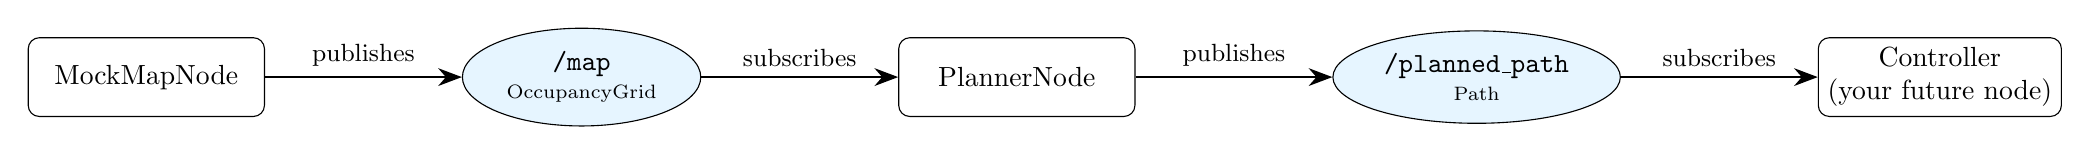
\begin{tikzpicture}[
    node distance=3cm,
    box/.style={rectangle, draw, rounded corners, minimum width=3cm, minimum height=1cm, align=center},
    topic/.style={ellipse, draw, fill=keybox, minimum width=2.5cm, align=center},
    arr/.style={-{Stealth[length=3mm]}, thick}
]
    \node[box] (mock) {MockMapNode};
    \node[topic, right=2.5cm of mock] (map) {\texttt{/map}\\[-2pt]\scriptsize OccupancyGrid};
    \node[box, right=2.5cm of map] (planner) {PlannerNode};

    \node[topic, right=2.5cm of planner] (path) {\texttt{/planned\_path}\\[-2pt]\scriptsize Path};
    \node[box, right=2.5cm of path] (control) {Controller\\(your future node)};

    \draw[arr] (mock) -- node[above, font=\small]{publishes} (map);
    \draw[arr] (map) -- node[above, font=\small]{subscribes} (planner);
    \draw[arr] (planner) -- node[above, font=\small]{publishes} (path);
    \draw[arr] (path) -- node[above, font=\small]{subscribes} (control);
\end{tikzpicture}
\caption{Data flow through topics in your system.}
\label{fig:topics}
\end{figure}

Here is how \texttt{mock\_map\_node.py} publishes the map:

\begin{lstlisting}[style=python, caption={Publishing a message (mock\_map\_node.py, simplified)}]
from nav_msgs.msg import OccupancyGrid

# In __init__:
self._pub = self.create_publisher(OccupancyGrid, '/map', qos)

# To publish:
msg = OccupancyGrid()
msg.info.width = 200
msg.info.height = 200
msg.info.resolution = 0.5
msg.data = grid.tolist()  # flat list of occupancy values
self._pub.publish(msg)
\end{lstlisting}

And here is how \texttt{planner\_node.py} subscribes to it:

\begin{lstlisting}[style=python, caption={Subscribing to a topic (planner\_node.py, simplified)}]
# In on_configure:
self._map_sub = self.create_subscription(
    OccupancyGrid,    # message type
    '/map',            # topic name
    self._on_map,      # callback function
    map_qos            # Quality of Service profile
)

def _on_map(self, msg: OccupancyGrid):
    """Called automatically whenever a new map is published."""
    self.get_logger().info(
        f'Map received: {msg.info.width}x{msg.info.height}'
    )
    # Convert OccupancyGrid data to our internal format
    self._build_planner(msg)
\end{lstlisting}

\begin{analogybox}[Analogy]
A topic is like a radio frequency. The mock map node \emph{broadcasts}
on frequency \texttt{/map}. The planner node \emph{tunes in} to that
frequency. If you later replace the mock with a real SLAM system, you
just make sure it broadcasts on the same frequency --- the planner
doesn't need to change at all.
\end{analogybox}

Your project has three topics:

\begin{center}
\begin{tabular}{llll}
    \toprule
    \textbf{Topic} & \textbf{Type} & \textbf{Publisher} & \textbf{Subscriber} \\
    \midrule
    \texttt{/map} & \texttt{OccupancyGrid} & mock\_map\_node (or SLAM) & planner\_node \\
    \texttt{/planned\_path} & \texttt{Path} & planner\_node & controller (future) \\
    \texttt{/planning\_stats} & \texttt{PlanningStats} & planner\_node & monitor (future) \\
    \bottomrule
\end{tabular}
\end{center}


% ======================================================================
\section{Actions: Request-Response for Long Tasks}
\label{sec:actions}
% ======================================================================

Topics are great for continuous data streams (like a map or sensor feed),
but planning is a \emph{one-shot, long-running} task: you send a start and
goal, wait for the planner to compute, and get a path back. Topics don't
naturally support this request-response pattern.

ROS\,2 provides \textbf{actions} for this. An action has three parts:

\begin{enumerate}[nosep]
    \item \textbf{Goal} --- what the client sends (the request)
    \item \textbf{Feedback} --- periodic updates while work is in progress
    \item \textbf{Result} --- what the server returns when done
\end{enumerate}

Your \texttt{PlanPath.action} defines all three:

\begin{lstlisting}[style=msg, caption={action/PlanPath.action}]
# Goal: what the client sends
geometry_msgs/PoseStamped start
geometry_msgs/PoseStamped goal
---
# Result: what the server returns
nav_msgs/Path path
PlanningStats stats
bool success
string message
---
# Feedback: updates during planning
string status
\end{lstlisting}

\begin{analogybox}[Analogy: Ordering Food]
An action is like ordering at a restaurant:
\begin{itemize}[nosep]
    \item \textbf{Goal}: ``I'd like a pizza with mushrooms'' (start + goal poses)
    \item \textbf{Feedback}: ``Your order is being prepared'' (status = ``planning'')
    \item \textbf{Result}: The pizza arrives (the planned path + statistics)
\end{itemize}
You can also \emph{cancel} the order (cancel the planning request).
\end{analogybox}

\subsection{Action Server (in planner\_node.py)}

The planner node creates an \textbf{action server} that waits for planning
requests:

\begin{lstlisting}[style=python, caption={Creating an action server (planner\_node.py)}]
from rclpy.action import ActionServer
from av_planner_interfaces.action import PlanPath

# In on_configure:
self._action_server = ActionServer(
    self,              # the node
    PlanPath,          # action type (auto-generated from .action file)
    '/plan_path',      # action name
    self._execute_plan # callback: what to do when a goal arrives
)
\end{lstlisting}

When a client sends a goal, ROS\,2 calls \texttt{\_execute\_plan}:

\begin{lstlisting}[style=python, caption={Action execute callback (planner\_node.py, simplified)}]
def _execute_plan(self, goal_handle):
    # 1. Extract start and goal from the request
    start = pose_to_state(goal_handle.request.start, CoreState)
    goal  = pose_to_state(goal_handle.request.goal, CoreState)

    # 2. Publish feedback
    feedback = PlanPath.Feedback()
    feedback.status = 'planning'
    goal_handle.publish_feedback(feedback)

    # 3. Run the actual Hybrid A* algorithm (pure Python, no ROS)
    plan_result = self._planner.plan(start, goal)

    # 4. Convert result to ROS messages and return
    result = PlanPath.Result()
    if plan_result is not None:
        path, info = plan_result
        result.path = states_to_path(path, 'map', stamp)
        result.success = True
        goal_handle.succeed()
    else:
        result.success = False
        goal_handle.abort()
    return result
\end{lstlisting}

\subsection{Action Client (how to send a goal)}

From the command line:

\begin{lstlisting}[style=bash, caption={Sending a planning goal via CLI}]
ros2 action send_goal /plan_path \
    av_planner_interfaces/action/PlanPath \
    "{start: {pose: {position: {x: 10.0, y: 50.0}, \
              orientation: {w: 1.0}}}, \
      goal: {pose: {position: {x: 90.0, y: 50.0}, \
             orientation: {w: 1.0}}}}"
\end{lstlisting}

Or from another Python node:

\begin{lstlisting}[style=python, caption={Sending a goal from Python (future mission planner)}]
from rclpy.action import ActionClient
from av_planner_interfaces.action import PlanPath

client = ActionClient(self, PlanPath, '/plan_path')
client.wait_for_server()

goal = PlanPath.Goal()
goal.start.pose.position.x = 10.0
goal.start.pose.position.y = 50.0
goal.start.pose.orientation.w = 1.0
goal.goal.pose.position.x = 90.0
goal.goal.pose.position.y = 50.0
goal.goal.pose.orientation.w = 1.0

future = client.send_goal_async(goal)
\end{lstlisting}

\subsection{Why Actions Instead of Topics?}

\begin{center}
\begin{tabular}{lll}
    \toprule
    & \textbf{Topic} & \textbf{Action} \\
    \midrule
    Pattern & Continuous stream & Request $\to$ response \\
    Blocking? & No (fire-and-forget) & Asynchronous (can await result) \\
    Feedback & No & Yes (periodic updates) \\
    Cancellation & No & Yes \\
    Use case & Map, sensor data & Planning, navigation goals \\
    \bottomrule
\end{tabular}
\end{center}

Planning is a perfect fit for actions because:
\begin{itemize}[nosep]
    \item It takes seconds (too long for a synchronous service call)
    \item The caller needs to know when it's done and whether it succeeded
    \item You might want to cancel a planning request mid-computation
\end{itemize}


% ======================================================================
\section{Lifecycle Nodes: Controlled Startup}
\label{sec:lifecycle}
% ======================================================================

A regular node starts doing everything the moment it launches.
A \textbf{lifecycle node} has explicit states and transitions, giving
you control over when things happen.

\subsection{Why?}

Consider this scenario: the planner node starts, but the map hasn't
arrived yet. With a regular node, you'd need manual checks everywhere
(``is the map ready? is the planner initialized?''). With a lifecycle
node, you keep the node in ``inactive'' state until everything is ready.

\subsection{State Machine}

\begin{figure}[h]
\centering
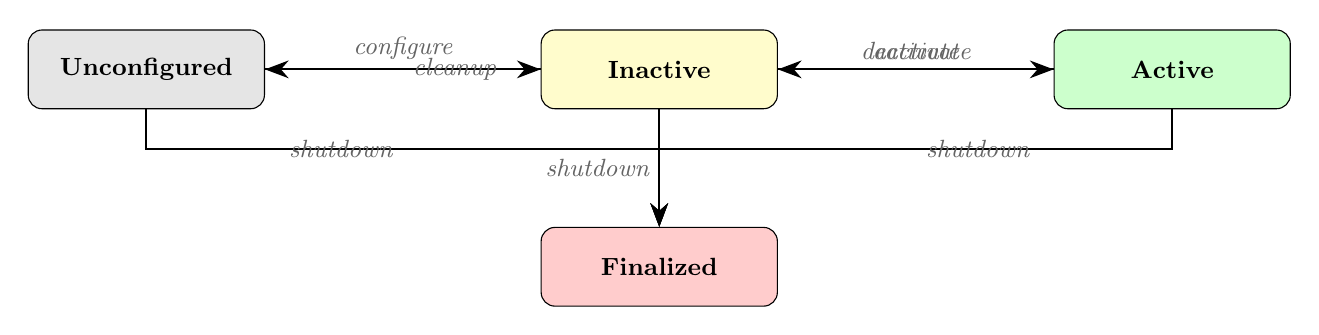
\begin{tikzpicture}[
    state/.style={rectangle, draw, rounded corners=5pt, minimum width=3cm,
                  minimum height=1cm, align=center, font=\small\bfseries},
    arr/.style={-{Stealth[length=3mm]}, thick},
    label/.style={font=\small\itshape, text=codegray}
]
    \node[state, fill=gray!20] (unconf) {Unconfigured};
    \node[state, fill=yellow!20, right=3.5cm of unconf] (inact) {Inactive};
    \node[state, fill=green!20, right=3.5cm of inact] (active) {Active};
    \node[state, fill=red!20, below=2cm of $(inact)$] (final) {Finalized};

    \draw[arr] (unconf) -- node[above, label] {configure} (inact);
    \draw[arr] (inact) -- node[above, label] {activate} (active);
    \draw[arr] (active) -- node[above, label] {deactivate} (inact);
    \draw[arr] (inact) -- node[right, label] {cleanup} (unconf);
    \draw[arr] (active.south) -- ++(0, -0.5) -| node[near start, right, label] {shutdown} (final);
    \draw[arr] (inact.south) -- node[left, label] {shutdown} (final);
    \draw[arr] (unconf.south) -- ++(0, -0.5) -| node[near start, left, label] {shutdown} (final);
\end{tikzpicture}
\caption{Lifecycle node state machine.}
\label{fig:lifecycle}
\end{figure}

\subsection{What Happens at Each Transition}

In \texttt{planner\_node.py}, each transition has a callback:

\begin{center}
\begin{tabular}{lp{9cm}}
    \toprule
    \textbf{Transition} & \textbf{What planner\_node does} \\
    \midrule
    \texttt{\_\_init\_\_} (constructor) & Declare parameters only. No publishers, no subscribers, nothing heavy. \\
    \texttt{on\_configure} & Import core algorithm classes, create the map subscriber, action server, and publishers. Node is now \emph{ready} but not processing. \\
    \texttt{on\_activate} & Log ``Activated. Ready for planning requests.'' Node starts accepting action goals. \\
    \texttt{on\_deactivate} & Log ``Deactivated.'' Temporarily stops accepting requests. \\
    \texttt{on\_cleanup} & Destroy all subscribers, publishers, action server. Release the planner. \\
    \bottomrule
\end{tabular}
\end{center}

\begin{lstlisting}[style=python, caption={Lifecycle callbacks (planner\_node.py)}]
from rclpy.lifecycle import Node as LifecycleNode, TransitionCallbackReturn

class PlannerNode(LifecycleNode):
    def __init__(self):
        super().__init__('planner_node')
        self._declare_params()          # Only declare parameters
        self._planner = None

    def on_configure(self, state):
        # Heavy setup: imports, subscribers, publishers, action server
        self._core_classes = _setup_core_imports(project_root)
        self._map_sub = self.create_subscription(...)
        self._action_server = ActionServer(...)
        self._path_pub = self.create_publisher(...)
        return TransitionCallbackReturn.SUCCESS

    def on_activate(self, state):
        self.get_logger().info('Ready for planning requests.')
        return super().on_activate(state)

    def on_cleanup(self, state):
        self.destroy_subscription(self._map_sub)
        self._action_server.destroy()
        self._planner = None
        return TransitionCallbackReturn.SUCCESS
\end{lstlisting}

\subsection{Transitioning from the Command Line}

After launching the node, you manually bring it to the active state:

\begin{lstlisting}[style=bash, caption={Lifecycle transitions}]
# Node starts in "unconfigured" state
ros2 lifecycle set /planner_node configure
# Now it creates subscribers, publishers, action server
# and starts listening for /map

ros2 lifecycle set /planner_node activate
# Now it accepts planning requests via /plan_path action
\end{lstlisting}


% ======================================================================
\section{Quality of Service (QoS): Delivery Guarantees}
\label{sec:qos}
% ======================================================================

QoS profiles control \emph{how} messages are delivered. The two most
important settings for your project:

\subsection{Reliability}

\begin{itemize}[nosep]
    \item \textbf{RELIABLE}: Every message is guaranteed to arrive
          (retransmission if needed). Used for map and path --- you cannot
          afford to miss these.
    \item \textbf{BEST\_EFFORT}: Messages may be dropped. Used for
          high-frequency sensor data where losing one frame is okay.
\end{itemize}

\subsection{Durability}

\begin{itemize}[nosep]
    \item \textbf{VOLATILE}: Only subscribers connected at the moment
          of publishing receive the message.
    \item \textbf{TRANSIENT\_LOCAL}: The publisher keeps the last
          message. New subscribers that connect \emph{later} still receive it.
\end{itemize}

\begin{keybox}[Why TRANSIENT\_LOCAL for /map?]
The mock map node publishes the map once. If \texttt{planner\_node}
starts \emph{after} the map was published, it would miss it with
VOLATILE durability. TRANSIENT\_LOCAL ensures the planner receives
the last published map even if it subscribes late. This is critical
because the map is published infrequently (once, then heartbeats every
10 seconds).
\end{keybox}

\begin{lstlisting}[style=python, caption={QoS profile for map subscription (planner\_node.py)}]
from rclpy.qos import QoSProfile, ReliabilityPolicy, DurabilityPolicy

map_qos = QoSProfile(
    reliability=ReliabilityPolicy.RELIABLE,       # don't drop
    durability=DurabilityPolicy.TRANSIENT_LOCAL,   # late joiners get it
    history=HistoryPolicy.KEEP_LAST,
    depth=1                                        # keep only latest map
)
\end{lstlisting}

\begin{center}
\begin{tabular}{llll}
    \toprule
    \textbf{Topic} & \textbf{Reliability} & \textbf{Durability} & \textbf{Why} \\
    \midrule
    \texttt{/map} & RELIABLE & TRANSIENT\_LOCAL & Map is critical, published rarely \\
    \texttt{/planned\_path} & RELIABLE & VOLATILE & Path consumed immediately \\
    \texttt{/planning\_stats} & RELIABLE & VOLATILE & Stats consumed immediately \\
    \bottomrule
\end{tabular}
\end{center}

\textbf{Important rule}: Publisher and subscriber QoS must be \emph{compatible}.
If the publisher is TRANSIENT\_LOCAL, the subscriber must also be
TRANSIENT\_LOCAL. Mismatched QoS is the \#1 cause of ``my subscriber
doesn't receive anything.''


% ======================================================================
\section{The Adapter Pattern: Connecting Algorithm to ROS}
\label{sec:adapters}
% ======================================================================

This is the central design pattern of your ROS\,2 package. The core
algorithm expects certain Python objects (\texttt{State}, \texttt{MapHandler}).
ROS\,2 provides different objects (\texttt{PoseStamped}, \texttt{OccupancyGrid}).
The \textbf{adapters} translate between them.

\begin{figure}[h]
\centering
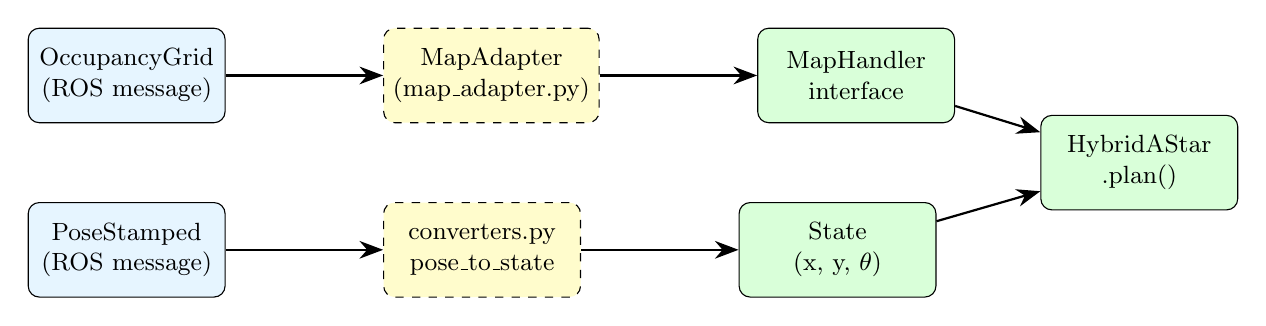
\begin{tikzpicture}[
    box/.style={rectangle, draw, rounded corners, minimum width=2.5cm, minimum height=1.2cm, align=center, font=\small},
    adapter/.style={box, fill=yellow!20, dashed},
    rosbox/.style={box, fill=keybox},
    algbox/.style={box, fill=green!15},
    arr/.style={-{Stealth[length=3mm]}, thick}
]
    % ROS side
    \node[rosbox] (occgrid) {OccupancyGrid\\(ROS message)};
    \node[rosbox, below=1cm of occgrid] (posestamped) {PoseStamped\\(ROS message)};

    % Adapters
    \node[adapter, right=2cm of occgrid] (mapadapt) {MapAdapter\\(map\_adapter.py)};
    \node[adapter, right=2cm of posestamped] (conv) {converters.py\\pose\_to\_state};

    % Algorithm side
    \node[algbox, right=2cm of mapadapt] (maphandler) {MapHandler\\interface};
    \node[algbox, right=2cm of conv] (state) {State\\(x, y, $\theta$)};

    \node[algbox, right=1.2cm of $(maphandler.east)!0.5!(state.east)$] (planner) {HybridAStar\\.plan()};

    \draw[arr] (occgrid) -- (mapadapt);
    \draw[arr] (mapadapt) -- (maphandler);
    \draw[arr] (posestamped) -- (conv);
    \draw[arr] (conv) -- (state);
    \draw[arr] (maphandler) -- (planner);
    \draw[arr] (state) -- (planner);
\end{tikzpicture}
\caption{Adapter pattern: ROS messages $\to$ adapters $\to$ algorithm objects.}
\label{fig:adapters}
\end{figure}

\subsection{Data Converter (converters.py)}
\label{sec:converters}

The converter functions translate between ROS\,2 message types and the
algorithm's \texttt{State} class. They contain \textbf{zero} algorithm logic ---
just data transformation.

\subsubsection{Quaternion $\leftrightarrow$ Yaw}

ROS\,2 represents orientation as a \textbf{quaternion} $(x, y, z, w)$ --- a
4D rotation representation. Your algorithm uses a single angle $\theta$
(yaw = rotation about the Z axis). The conversion is:

\begin{equation}
\theta = \text{atan2}\!\left(2(wz + xy),\; 1 - 2(y^2 + z^2)\right)
\end{equation}

For 2D (no pitch or roll), $x = y = 0$, so this simplifies to
$z = \sin(\theta/2)$, $w = \cos(\theta/2)$.

\begin{lstlisting}[style=python, caption={Quaternion conversion (converters.py)}]
def yaw_from_quaternion(q):
    siny_cosp = 2.0 * (q.w * q.z + q.x * q.y)
    cosy_cosp = 1.0 - 2.0 * (q.y * q.y + q.z * q.z)
    return math.atan2(siny_cosp, cosy_cosp)

def quaternion_from_yaw(yaw):
    q = Quaternion()
    q.z = math.sin(yaw / 2.0)
    q.w = math.cos(yaw / 2.0)
    return q
\end{lstlisting}

\subsubsection{PoseStamped $\to$ State}

\begin{lstlisting}[style=python, caption={Converting a ROS pose to algorithm State}]
def pose_to_state(msg: PoseStamped, state_cls):
    x = msg.pose.position.x        # meters
    y = msg.pose.position.y        # meters
    theta = yaw_from_quaternion(msg.pose.orientation)  # radians
    return state_cls(x, y, theta)   # State(x, y, theta)
\end{lstlisting}

Note that \texttt{state\_cls} is passed as a parameter --- the converter
file \emph{never} imports from \texttt{src/}. This keeps the adapter
layer free from any dependency on the algorithm code.

\subsubsection{List of States $\to$ nav\_msgs/Path}

After planning, the algorithm returns a list of \texttt{State} objects.
We convert each to a \texttt{PoseStamped} and pack them into a \texttt{Path}:

\begin{lstlisting}[style=python, caption={Converting algorithm output to a ROS Path}]
def states_to_path(states, frame_id, stamp):
    path_msg = Path()
    path_msg.header.frame_id = frame_id  # "map"
    path_msg.header.stamp = stamp
    for s in states:
        path_msg.poses.append(state_to_pose(s, frame_id, stamp))
    return path_msg
\end{lstlisting}

% ------------------------------------------------------------------
\subsection{Map Adapter (map\_adapter.py)}
\label{sec:mapadapter}

This is the most important adapter. Your Hybrid A* algorithm expects a
\texttt{MapHandler} object (from \texttt{src/map\_handler.py}) which provides:
\begin{itemize}[nosep]
    \item \texttt{map\_data} --- 2D numpy array (0=free, 1=obstacle)
    \item \texttt{width}, \texttt{height} --- map dimensions in meters
    \item \texttt{resolution} --- meters per cell
    \item \texttt{cost\_field} --- distance-based cost field
    \item \texttt{world\_to\_pixel(x, y)} --- coordinate conversion
    \item \texttt{is\_obstacle\_world(x, y)} --- collision check
    \item \texttt{is\_collision(points)} --- check multiple points
    \item etc.
\end{itemize}

In the standalone Python planner, \texttt{MapHandler} loads a PNG image.
In ROS\,2, maps arrive as \texttt{OccupancyGrid} messages. The \textbf{MapAdapter}
creates an object with the \emph{same interface} as \texttt{MapHandler}
but initializes from ROS data instead of a PNG file.

\begin{lstlisting}[style=python, caption={MapAdapter constructor (map\_adapter.py, simplified)}]
class MapAdapter:
    def __init__(self, data, resolution, width, height,
                 origin_x=0.0, origin_y=0.0, obstacle_threshold=50):
        self.resolution = resolution
        self.pixel_width = width
        self.pixel_height = height

        # Convert OccupancyGrid values to binary:
        #   OccupancyGrid: -1=unknown, 0=free, 100=occupied
        #   MapHandler:    0=free, 1=obstacle
        grid = np.array(data, dtype=np.int8).reshape((height, width))
        self.map_data = np.where(
            (grid >= obstacle_threshold) | (grid < 0), 1, 0
        ).astype(np.uint8)

        self.width  = width * resolution    # meters
        self.height = height * resolution   # meters

        # Compute the same cost field as MapHandler
        self._compute_cost_field()
\end{lstlisting}

\begin{keybox}[Duck Typing]
Python uses \textbf{duck typing}: ``if it walks like a duck and quacks
like a duck, it's a duck.'' \texttt{MapAdapter} doesn't inherit from
\texttt{MapHandler}. It just has the same methods and attributes.
When \texttt{HybridAStar} calls \texttt{map\_handler.is\_collision(points)},
Python doesn't check the type --- it just looks for a method named
\texttt{is\_collision}. Since \texttt{MapAdapter} has one, it works.
\end{keybox}

\subsubsection{OccupancyGrid Data Format}

The OccupancyGrid uses a different value convention than your PNG maps:

\begin{center}
\begin{tabular}{ccc}
    \toprule
    \textbf{Source} & \textbf{Free} & \textbf{Occupied} \\
    \midrule
    PNG image & 255 (white) & 0 (black) \\
    OccupancyGrid & 0 & 100 \\
    MapHandler internal & 0 & 1 \\
    \bottomrule
\end{tabular}
\end{center}

The MapAdapter handles this conversion. It also treats ``unknown'' cells
($-1$) as obstacles for safety.

\subsubsection{Cost Field Computation}

Both \texttt{MapHandler} and \texttt{MapAdapter} compute a cost field
using \textbf{Euclidean distance transform}. For each free cell, the cost
is inversely proportional to its distance from the nearest obstacle.
Cells far from obstacles have low cost; cells near obstacles have high
cost. This encourages the planner to prefer paths away from walls.

\begin{lstlisting}[style=python, caption={Cost field computation (map\_adapter.py)}]
from scipy.ndimage import distance_transform_edt

def _compute_cost_field(self):
    free_space = (1 - self.map_data).astype(np.float64)
    self.distance_field = distance_transform_edt(free_space)
    max_dist = self.distance_field.max()
    if max_dist > 0:
        self.cost_field = 1.0 - np.clip(
            self.distance_field / max_dist, 0.0, 1.0
        )
    else:
        self.cost_field = np.zeros_like(self.map_data, dtype=np.float64)
\end{lstlisting}

% ======================================================================
\section{Parameters: Configuration Without Recompiling}
\label{sec:params}
% ======================================================================

ROS\,2 nodes can declare \textbf{parameters} --- named values that can be
set from YAML files, command line, or changed at runtime. This replaces
hardcoded constants.

\subsection{Declaring Parameters}

In the constructor, the planner declares every configurable value:

\begin{lstlisting}[style=python, caption={Parameter declaration (planner\_node.py)}]
def _declare_params(self):
    self.declare_parameter('frame_id', 'map')        # string
    self.declare_parameter('vehicle.wheel_base', 2.5) # float
    self.declare_parameter('motion.max_steering_angle', 40.0)
    self.declare_parameter('search.xy_resolution', 1.0)
    self.declare_parameter('cost.steering_penalty', 1.5)
    # ... etc.
\end{lstlisting}

The second argument is the default value. The actual value comes from
\texttt{params.yaml} at launch time.

\subsection{Reading Parameters}

When building the planner, each parameter is read and passed to the
algorithm constructor:

\begin{lstlisting}[style=python, caption={Reading parameters to construct planner}]
motion_model = MotionModel(
    wheel_base=self.get_parameter('vehicle.wheel_base').value,
    max_steering_angle=self.get_parameter('motion.max_steering_angle').value,
    step_size=self.get_parameter('motion.step_size').value,
)
\end{lstlisting}

\subsection{The params.yaml File}

All parameter values live in a single YAML file loaded at launch:

\begin{lstlisting}[style=yaml, caption={config/params.yaml (excerpt)}]
planner_node:
  ros__parameters:
    frame_id: "map"
    project_root: "/path/to/hybrid_astar_planner"

    vehicle:
      wheel_base: 2.5       # meters
      length: 4.5
      width: 2.0

    motion:
      max_steering_angle: 40.0   # degrees
      step_size: 2.0             # meters
      num_steering_angles: 5

    cost:
      steering_penalty: 1.5
      reversing_penalty: 2.0
      direction_switch_penalty: 10.0

    heuristic:
      type: "max"    # h = max(RS distance, 2D Dijkstra)
      turning_radius: 2.98
\end{lstlisting}

The YAML nesting (e.g., \texttt{vehicle: \{wheel\_base: 2.5\}}) becomes
a dotted parameter name (\texttt{vehicle.wheel\_base}). The top-level key
\texttt{planner\_node:} matches the node name, and \texttt{ros\_\_parameters:}
(with double underscores) is the required ROS\,2 prefix.


% ======================================================================
\section{The Complete Data Flow}
\label{sec:dataflow}
% ======================================================================

Now let's trace a complete planning request through the system, from
map arrival to path publication.

\subsection{Step 1: Map Arrives}

\begin{enumerate}[nosep]
    \item \texttt{mock\_map\_node} loads a PNG image (\texttt{maps/map\_open.png})
    \item It converts the image to an \texttt{OccupancyGrid} message
          (flips vertically, thresholds pixels to 0/100)
    \item It publishes the message on \texttt{/map} with TRANSIENT\_LOCAL QoS
\end{enumerate}

\subsection{Step 2: Planner Receives Map}

\begin{enumerate}[nosep]
    \item \texttt{planner\_node}'s \texttt{\_on\_map} callback fires
    \item It creates a \texttt{MapAdapter} from the OccupancyGrid data
    \item It builds the \emph{entire} planner pipeline:
    \begin{itemize}[nosep]
        \item \texttt{MapAdapter} $\to$ \texttt{MotionModel} $\to$
              \texttt{VehicleFootprint} $\to$ \texttt{HeuristicCalculator}
              $\to$ \texttt{HybridAStar}
    \end{itemize}
    \item Stores the planner in \texttt{self.\_planner}
\end{enumerate}

\begin{lstlisting}[style=python, caption={Planner pipeline construction (planner\_node.py)}]
def _build_planner(self, msg: OccupancyGrid):
    # Create map adapter (replaces MapHandler's PNG loading)
    self._map_handler = MapAdapter(
        data=np.array(msg.data, dtype=np.int8),
        resolution=msg.info.resolution,
        width=msg.info.width,
        height=msg.info.height,
    )

    # Build motion model (bicycle kinematics)
    motion_model = MotionModel(wheel_base=..., ...)

    # Build heuristic: h = max(RS distance, 2D Dijkstra)
    heuristic = HeuristicCalculator(
        map_handler=self._map_handler,  # MapAdapter works here!
        heuristic_type='max',
    )

    # Build planner: f = g + h, with cost penalties
    self._planner = HybridAStar(
        map_handler=self._map_handler,
        motion_model=motion_model,
        heuristic_calculator=heuristic,
        steering_penalty=1.5,
        reversing_penalty=2.0,
        # ...
    )
\end{lstlisting}

\subsection{Step 3: Planning Request}

\begin{enumerate}[nosep]
    \item A client sends a \texttt{PlanPath} goal with start and goal poses
    \item \texttt{\_execute\_plan} callback fires
    \item Converts \texttt{PoseStamped} $\to$ \texttt{State} using \texttt{pose\_to\_state}
    \item Calls \texttt{self.\_planner.plan(start, goal)} --- pure Python, no ROS
    \item The algorithm runs: bicycle kinematics, A* search, Reeds-Shepp shots
    \item Returns \texttt{(path, info)} where \texttt{path} is a list of \texttt{State}
\end{enumerate}

\subsection{Step 4: Result Returned}

\begin{enumerate}[nosep]
    \item Converts \texttt{List[State]} $\to$ \texttt{nav\_msgs/Path} using \texttt{states\_to\_path}
    \item Fills \texttt{PlanningStats} from the info dict
    \item Publishes path on \texttt{/planned\_path} and stats on \texttt{/planning\_stats}
    \item Returns \texttt{PlanPath.Result} to the action client
\end{enumerate}

\begin{figure}[h]
\centering
\begin{tikzpicture}[
    step/.style={rectangle, draw, rounded corners=3pt, minimum width=6cm, minimum height=0.8cm, align=center, font=\small},
    arr/.style={-{Stealth[length=2.5mm]}, thick},
    note/.style={font=\scriptsize\itshape, text=codegray}
]
    \node[step, fill=keybox] (s1) {PNG $\to$ OccupancyGrid \textit{(mock\_map\_node)}};
    \node[step, fill=yellow!15, below=0.5cm of s1] (s2) {OccupancyGrid $\to$ MapAdapter \textit{(map\_adapter.py)}};
    \node[step, fill=green!15, below=0.5cm of s2] (s3) {MapAdapter $\to$ MotionModel $\to$ HybridAStar};
    \node[step, fill=keybox, below=0.5cm of s3] (s4) {PoseStamped $\to$ State \textit{(converters.py)}};
    \node[step, fill=green!15, below=0.5cm of s4] (s5) {\texttt{planner.plan(start, goal)} \textit{(pure Python)}};
    \node[step, fill=yellow!15, below=0.5cm of s5] (s6) {List[State] $\to$ Path \textit{(converters.py)}};
    \node[step, fill=keybox, below=0.5cm of s6] (s7) {Publish \texttt{/planned\_path} + \texttt{/planning\_stats}};

    \draw[arr] (s1) -- (s2);
    \draw[arr] (s2) -- (s3);
    \draw[arr] (s3) -- (s4);
    \draw[arr] (s4) -- (s5);
    \draw[arr] (s5) -- (s6);
    \draw[arr] (s6) -- (s7);

    \node[note, right=0.3cm of s1] {ROS message};
    \node[note, right=0.3cm of s2] {adapter};
    \node[note, right=0.3cm of s3] {algorithm setup};
    \node[note, right=0.3cm of s4] {adapter};
    \node[note, right=0.3cm of s5] {algorithm runs};
    \node[note, right=0.3cm of s6] {adapter};
    \node[note, right=0.3cm of s7] {ROS message};
\end{tikzpicture}
\caption{Complete data flow: from PNG to published path.}
\label{fig:dataflow}
\end{figure}


% ======================================================================
\section{Concurrency: Callback Groups and Executors}
\label{sec:concurrency}
% ======================================================================

By default, ROS\,2 processes callbacks \emph{one at a time} (single-threaded).
This means if the planner is computing a path (which takes seconds),
an incoming map update would have to wait. Your node solves this
with two mechanisms.

\subsection{Callback Groups}

A \textbf{callback group} defines which callbacks can run concurrently:

\begin{lstlisting}[style=python, caption={Callback groups (planner\_node.py)}]
self._map_cb_group = MutuallyExclusiveCallbackGroup()
self._action_cb_group = MutuallyExclusiveCallbackGroup()

self._map_sub = self.create_subscription(
    OccupancyGrid, '/map', self._on_map, map_qos,
    callback_group=self._map_cb_group     # group 1
)
self._action_server = ActionServer(
    self, PlanPath, '/plan_path', self._execute_plan,
    callback_group=self._action_cb_group  # group 2
)
\end{lstlisting}

Callbacks in \emph{different} groups can run at the same time.
Callbacks in the \emph{same} group never overlap (mutually exclusive).

This means: a map update and a planning request can run concurrently,
but two map updates cannot (which is what we want).

\subsection{MultiThreadedExecutor}

To actually run callbacks concurrently, we need multiple threads:

\begin{lstlisting}[style=python, caption={Multi-threaded executor (planner\_node.py)}]
from rclpy.executors import MultiThreadedExecutor

executor = MultiThreadedExecutor(num_threads=2)
executor.add_node(node)
executor.spin()  # dispatches callbacks to threads
\end{lstlisting}

\subsection{Thread Safety: The Lock}

Since the map callback and planning callback can run simultaneously,
we need a lock to prevent them from accessing the planner at the
same time:

\begin{lstlisting}[style=python, caption={Thread safety with a lock}]
self._plan_lock = threading.Lock()

def _on_map(self, msg):
    with self._plan_lock:       # acquire lock
        self._build_planner(msg) # rebuild planner

def _execute_plan(self, goal_handle):
    with self._plan_lock:       # acquire same lock
        result = self._planner.plan(start, goal)
\end{lstlisting}

This ensures the planner is never being used while it's being rebuilt.


% ======================================================================
\section{Package Structure and Build System}
\label{sec:packages}
% ======================================================================

\subsection{Why Two Packages?}

\begin{center}
\begin{tabular}{llp{7cm}}
    \toprule
    \textbf{Package} & \textbf{Build Type} & \textbf{Contents} \\
    \midrule
    \texttt{av\_planner\_interfaces} & CMake & Custom message (\texttt{.msg}) and action (\texttt{.action}) definitions. CMake is required because the ROS\,2 code generator (\texttt{rosidl}) needs CMake to generate Python bindings from \texttt{.msg}/\texttt{.action} files. \\[4pt]
    \texttt{av\_planner} & Python (\texttt{ament\_python}) & Your actual nodes, adapters, launch file, config. Pure Python. \\
    \bottomrule
\end{tabular}
\end{center}

\subsection{Workspace Layout}

\begin{lstlisting}[style=bash, caption={Directory structure}]
ros2_ws/
  src/
    av_planner_interfaces/    # Package 1: interfaces (CMake)
      package.xml
      CMakeLists.txt
      msg/PlanningStats.msg
      action/PlanPath.action

    av_planner/               # Package 2: nodes (Python)
      package.xml
      setup.py
      setup.cfg
      resource/av_planner     # empty marker (ament requirement)
      config/params.yaml
      launch/planner.launch.xml
      av_planner/             # Python module
        __init__.py
        adapters/
          __init__.py
          map_adapter.py
          converters.py
        nodes/
          __init__.py
          planner_node.py
          mock_map_node.py
\end{lstlisting}

\subsection{package.xml: The Manifest}

Every ROS\,2 package has a \texttt{package.xml} that declares its name,
dependencies, and build type:

\begin{lstlisting}[style=xml, caption={av\_planner/package.xml (key parts)}]
<package format="3">
  <name>av_planner</name>
  <buildtool_depend>ament_python</buildtool_depend>

  <depend>rclpy</depend>              <!-- ROS Python client -->
  <depend>nav_msgs</depend>           <!-- OccupancyGrid, Path -->
  <depend>geometry_msgs</depend>      <!-- PoseStamped -->
  <depend>av_planner_interfaces</depend>  <!-- our custom msgs -->

  <export>
    <build_type>ament_python</build_type>
  </export>
</package>
\end{lstlisting}

\subsection{setup.py: Python Entry Points}

The \texttt{entry\_points} section tells ROS\,2 which functions to expose
as executable commands:

\begin{lstlisting}[style=python, caption={setup.py entry points}]
entry_points={
    'console_scripts': [
        'planner_node = av_planner.nodes.planner_node:main',
        'mock_map_node = av_planner.nodes.mock_map_node:main',
    ],
},
\end{lstlisting}

This means \texttt{ros2 run av\_planner planner\_node} calls the
\texttt{main()} function in \texttt{av\_planner/nodes/planner\_node.py}.

\subsection{Building}

\begin{lstlisting}[style=bash, caption={Build and source}]
cd ros2_ws
source /opt/ros/humble/setup.bash   # load ROS 2 base
colcon build --symlink-install       # build all packages
source install/setup.bash            # load your packages
\end{lstlisting}

\texttt{colcon build} does two things:
\begin{enumerate}[nosep]
    \item For \texttt{av\_planner\_interfaces}: runs the \texttt{rosidl}
          code generator to produce Python classes from \texttt{.msg}
          and \texttt{.action} files.
    \item For \texttt{av\_planner}: installs the Python package and
          registers the entry points.
\end{enumerate}

\texttt{--symlink-install} creates symlinks instead of copies, so you
can edit Python files without rebuilding (you still need to rebuild
if you change \texttt{.msg} or \texttt{.action} files).


% ======================================================================
\section{Launch Files: Starting Multiple Nodes}
\label{sec:launch}
% ======================================================================

A \textbf{launch file} starts multiple nodes at once with their
configuration. Your launch file is in XML format:

\begin{lstlisting}[style=xml, caption={launch/planner.launch.xml}]
<launch>
  <arg name="params_file"
       default="$(find-pkg-share av_planner)/config/params.yaml"/>
  <arg name="use_mock_map" default="true"/>

  <!-- Only start mock map if use_mock_map is true -->
  <group if="$(var use_mock_map)">
    <node pkg="av_planner" exec="mock_map_node"
          name="mock_map_node" output="screen">
      <param from="$(var params_file)"/>
    </node>
  </group>

  <!-- Always start the planner -->
  <node pkg="av_planner" exec="planner_node"
        name="planner_node" output="screen">
    <param from="$(var params_file)"/>
  </node>
</launch>
\end{lstlisting}

\subsection{Key Elements}

\begin{description}[nosep, style=nextline]
    \item[\texttt{<arg>}] Defines a launch argument. \texttt{use\_mock\_map}
    defaults to \texttt{true} but can be overridden:
    \begin{lstlisting}[style=bash]
ros2 launch av_planner planner.launch.xml use_mock_map:=false
    \end{lstlisting}

    \item[\texttt{<group if=...>}] Conditionally includes nodes.
    When connecting to a real SLAM system, you set \texttt{use\_mock\_map:=false}
    to skip the mock.

    \item[\texttt{<node>}] Starts a node.
    \texttt{pkg} = package name, \texttt{exec} = entry point name,
    \texttt{name} = ROS node name.

    \item[\texttt{<param from=...>}] Loads parameters from a YAML file.
    \texttt{\$(find-pkg-share av\_planner)} resolves to the package's
    \texttt{share/} directory where \texttt{params.yaml} was installed.
\end{description}


% ======================================================================
\section{How Core Imports Work}
\label{sec:imports}
% ======================================================================

The core algorithm files (\texttt{src/hybrid\_astar/}) are \emph{not}
inside the ROS\,2 package. They sit in the project root:

\begin{lstlisting}[style=bash]
hybrid_astar_planner/
  src/                    # Core algorithm (NOT a ROS package)
    state.py
    map_handler.py
    hybrid_astar/
      hybrid_astar.py
      motion_model.py
      heuristic.py
      reeds_shepp.py
  ros2_ws/src/            # ROS 2 packages (middleware only)
    av_planner/...
\end{lstlisting}

The planner node imports these at configuration time using a
\texttt{project\_root} parameter:

\begin{lstlisting}[style=python, caption={Dynamic core imports (planner\_node.py)}]
def _setup_core_imports(project_root: str):
    """Add project root to sys.path so 'from src.*' imports resolve."""
    if project_root not in sys.path:
        sys.path.insert(0, project_root)

    from src.state import State as CoreState
    from src.hybrid_astar.motion_model import MotionModel, VehicleFootprint
    from src.hybrid_astar.heuristic import HeuristicCalculator
    from src.hybrid_astar.hybrid_astar import HybridAStar

    return CoreState, MotionModel, VehicleFootprint, HeuristicCalculator, HybridAStar
\end{lstlisting}

This design means:
\begin{itemize}[nosep]
    \item The core algorithm has \textbf{zero ROS dependencies} --- it can
          run standalone via \texttt{main.py}
    \item The ROS node is a \textbf{thin wrapper} --- it just translates
          data formats and manages communication
    \item If you improve the algorithm, you don't need to touch the ROS code
    \item If you change the ROS interface, you don't need to touch the algorithm
\end{itemize}


% ======================================================================
\section{Putting It All Together: Step by Step}
\label{sec:tutorial}
% ======================================================================

Here is the complete sequence to run the planner:

\subsection{Build}

\begin{lstlisting}[style=bash]
cd ~/Documents/hybrid_astar_planner/ros2_ws
source /opt/ros/humble/setup.bash
colcon build --symlink-install
source install/setup.bash
\end{lstlisting}

\subsection{Launch}

\begin{lstlisting}[style=bash]
ros2 launch av_planner planner.launch.xml
\end{lstlisting}

This starts \texttt{mock\_map\_node} and \texttt{planner\_node}.
The mock node immediately publishes the map. The planner node starts
in ``unconfigured'' state.

\subsection{Configure and Activate}

\begin{lstlisting}[style=bash]
ros2 lifecycle set /planner_node configure
# -> Imports core classes, creates subscribers/publishers/action server
# -> Receives map from /map, builds planner pipeline

ros2 lifecycle set /planner_node activate
# -> "Activated. Ready for planning requests."
\end{lstlisting}

\subsection{Plan}

\begin{lstlisting}[style=bash]
ros2 action send_goal /plan_path av_planner_interfaces/action/PlanPath \
  "{start: {pose: {position: {x: 10.0, y: 50.0}, \
            orientation: {w: 1.0}}}, \
    goal: {pose: {position: {x: 90.0, y: 50.0}, \
           orientation: {w: 1.0}}}}"
\end{lstlisting}

\subsection{Verify}

\begin{lstlisting}[style=bash]
ros2 topic echo /planned_path --once     # see the path
ros2 topic echo /planning_stats --once   # see the metrics
\end{lstlisting}

\subsection{Useful Debugging Commands}

\begin{lstlisting}[style=bash]
ros2 node list              # list all running nodes
ros2 topic list             # list all active topics
ros2 topic info /map        # show publishers/subscribers
ros2 param list /planner_node  # list all parameters
ros2 param get /planner_node vehicle.wheel_base  # read a param
ros2 lifecycle get /planner_node  # current lifecycle state
\end{lstlisting}


% ======================================================================
\section{Integration with Real Systems}
\label{sec:integration}
% ======================================================================

The entire ROS\,2 package is designed so that replacing the mock
with real components requires \textbf{zero code changes}:

\begin{center}
\begin{tabular}{lp{5cm}p{5cm}}
    \toprule
    \textbf{Component} & \textbf{Standalone (testing)} & \textbf{Real System} \\
    \midrule
    Map source & \texttt{mock\_map\_node} (PNG) & SLAM / \texttt{map\_server} \\
    Planning input & CLI action goal & Mission planner node \\
    Path consumer & \texttt{ros2 topic echo} & Controller node \\
    \bottomrule
\end{tabular}
\end{center}

To switch to a real system:

\begin{lstlisting}[style=bash]
# Don't start mock map - real SLAM publishes on /map
ros2 launch av_planner planner.launch.xml use_mock_map:=false
\end{lstlisting}

As long as your SLAM system publishes \texttt{nav\_msgs/OccupancyGrid}
on \texttt{/map}, and your mission planner sends goals via the
\texttt{/plan\_path} action, the planner works identically.


% ======================================================================
\section{Summary of Key Concepts}
\label{sec:summary}
% ======================================================================

\begin{center}
\begin{tabular}{lp{10cm}}
    \toprule
    \textbf{Concept} & \textbf{In Your Project} \\
    \midrule
    \textbf{Node} & \texttt{planner\_node}, \texttt{mock\_map\_node} --- independent programs \\
    \textbf{Topic} & \texttt{/map}, \texttt{/planned\_path}, \texttt{/planning\_stats} --- named channels \\
    \textbf{Message} & \texttt{OccupancyGrid}, \texttt{Path}, \texttt{PlanningStats} --- structured data \\
    \textbf{Action} & \texttt{/plan\_path} --- request/feedback/result for planning \\
    \textbf{Lifecycle} & Unconfigured $\to$ Inactive $\to$ Active --- controlled startup \\
    \textbf{QoS} & TRANSIENT\_LOCAL for map, RELIABLE for everything \\
    \textbf{Parameters} & \texttt{params.yaml} --- all algorithm settings \\
    \textbf{Adapter} & \texttt{MapAdapter}, \texttt{converters.py} --- translate ROS $\leftrightarrow$ algorithm \\
    \textbf{Launch} & \texttt{planner.launch.xml} --- starts everything with one command \\
    \textbf{Callback groups} & Separate groups for map and planning --- concurrent execution \\
    \textbf{Executor} & \texttt{MultiThreadedExecutor} --- enables concurrency \\
    \bottomrule
\end{tabular}
\end{center}

\vspace{1em}

\begin{keybox}[The Big Picture]
Your Hybrid A* algorithm is \textbf{100\% pure Python} with zero ROS imports.
The ROS\,2 package is a \textbf{thin middleware layer} that:
\begin{enumerate}[nosep]
    \item Receives map data from other modules (via topics)
    \item Translates it into the format your algorithm expects (via adapters)
    \item Runs your algorithm (one function call: \texttt{planner.plan()})
    \item Translates the result back to ROS messages (via adapters)
    \item Publishes the result for other modules to consume (via topics)
\end{enumerate}
That's it. ROS\,2 is the plumbing; your algorithm is the engine.
\end{keybox}


\end{document}
